\let\lesson\undefined
\newcommand{\lesson}{\phantomlesson{Ôn tập chương 5}}
\setcounter{section}{2}
\ANSMCQ
{	\begin{center}
		\begin{tabular}{|m{2.8em}|m{2.8em}|m{2.8em}|m{2.8em}|m{2.8em}|m{2.8em}|m{2.8em}|m{2.8em}|m{2.8em}|m{2.8em}|}
			\hline
			1.B  & 2.A  & 3.B & 4.B & 5.A  & 6.D & 7.A & 8.C & 9.C & 10.A  \\
			\hline
			11.C  & 12.C  & 13.A & 14.C & 15.D  & 16.A & 17.C & 18.A & 19.B & 20.B  \\
			\hline
			21.B  & 22.A  & 23.A & 24.C & 25.B  & 26.B & 27.A & 28.D & 29.A & 30.B  \\
			\hline
		\end{tabular}
	\end{center}
}
\begin{enumerate}[label=\bfseries Câu \arabic*:, leftmargin=1.5cm]
	\item \mkstar{1}\\
	{Đơn vị của moment lực là
		\begin{mcq}(4)
			\item $\si{\meter/\second}$.
			\item $\si{\newton\cdot\meter}$.
			\item $\si{\kilogram\cdot\meter}$.
			\item $\si{\newton\cdot\kilogram}$.
		\end{mcq}
	
}
\hideall{
\textbf{Đáp án B.}
}

\item \mkstar{1}\\
{Moment lực tác dụng lên vật là đại lượng
	\begin{mcq}
		\item đặc trưng cho tác dụng làm quay vật của lực.
		\item vô hướng.
		\item để xác định độ lớn của lực tác dụng.
		\item luôn có giá trị dương.
	\end{mcq}

}
\hideall{
\textbf{Đáp án A.}
}

\item \mkstar{1}\\
{Moment lực tác dụng lên một vật có trục quay cố định là đại lượng 
	\begin{mcq}
		\item đặc trưng cho tác dụng làm quay vật của lực và được đo bằng tích số của lực với khoảng cách từ điểm đặt lực đến trục quay. 
		\item đặc trưng cho tác dụng làm quay vật của lực và được đo bằng tích của lực và cánh tay đòn của nó. 
		\item đặc trưng cho độ mạnh yếu của lực. 
		\item luôn có giá trị âm.
	\end{mcq}

}
\hideall{
\textbf{Đáp án B.}
}

\item \mkstar{1}\\
{Theo quy tắc hợp lực song song cùng chiều. Điểm đặt của hợp lực được xác định dựa trên biểu thức sau 
	\begin{mcq}(4)
		\item $\dfrac{F_1}{F_2}=\dfrac{d_1}{d_2}$.
		\item $\dfrac{F_1}{F_2}=\dfrac{d_2}{d_1}$.
		\item $\dfrac{F_2}{F_1}=\dfrac{d_2}{d_2+d_1}$.
		\item $\dfrac{F_2}{F_1}=\dfrac{d_1}{d_2+d_1}$.
	\end{mcq}
}
\hideall{
	\textbf{Đáp án B.}
}

\item \mkstar{1}\\
{Phát biểu nào sau đây đúng với quy tắc moment lực?
\begin{mcq}
	\item Muốn cho một vật có trục quay cố định nằm cân bằng thì tổng moment của các lực có khuynh hướng làm vật quay theo một chiều phải bằng tổng moment của các lực có khuynh hướng làm vật quay theo chiều ngược lại.
	\item Muốn cho một vật có trục quay cố định nằm cân bằng thì tổng moment của các lực phải bằng hằng số.
	\item Muốn cho một vật có trục quay cố định nằm cân bằng thì tổng moment của các lực phải khác không.
	\item Muốn cho một vật có trục quay cố định nằm cân bằng thì tổng moment của các lực phải là một vector có giá đi qua trục quay. 
\end{mcq}
}
\hideall{
\textbf{Đáp án A.}
}

\item \mkstar{2}\\
{Lực có tác dụng làm cho vật rắn quay quanh một trục khi
\begin{mcq}
	\item lực có giá nằm trong mặt phẳng vuông góc với trục quay và cắt trục quay
	\item lực có giá song song với trục quay
	\item lực có giá cắt trục quay.
	\item lực có giá nằm trong mặt phẳng vuông góc với trục quay và không cắt trục quay.
	
\end{mcq}
}
\hideall{
\textbf{Đáp án D.}
}

\item \mkstar{2}\\
{Nhận xét nào sau đây về ngẫu lực là không chính xác?
	\begin{mcq}
		\item Hợp lực của ngẫu lực tuân theo quy tắc tổng hợp hai lực song song, ngược chiều.
		\item Ngẫu lực là hệ gồm hai lực song song, ngược chiều và có độ lớn bằng nhau.
		\item Moment của ngẫu lực tính theo công thức $M=F\cdot d$ (trong đó $d$ là cánh tay đòn của ngẫu lực).
		\item Nếu vật không có trục quay cố định chịu tác dụng của ngẫu lực thì nó sẽ quay quanh một trục đi qua trọng tâm và vuông góc với mặt phẳng chứa ngẫu lực.
	\end{mcq}

}
\hideall{
\textbf{Đáp án A.}\\
Ngẫu lực không có hợp lực vì không thể tìm được 1 lực duy nhất thay thế tác dụng của ngẫu lực.
}

\item \mkstar{2}\\
{Điều kiện để một vật nằm cân bằng là
	\begin{mcq}
		\item Tổng moment lực tác dụng lên vật phải bằng không.
		\item Hợp lực tác dụng lên vật phải bằng không.
		\item Hợp lực tác dụng lên vật phải bằng không và tổng moment lực tác dụng lên vật phải bằng không.
		\item Trọng lực và phản lực có nó phải cân bằng nhau.
	\end{mcq}
}
\hideall{
\textbf{Đáp án C.}
}



\item\mkstar{2}\\
{Người làm xiếc đi trên dây thường cầm một cây gậy nặng để làm gì?
	\begin{mcq}
		\item Để vừa đi vừa biểu diễn cho đẹp.
		\item Để tăng lực ma sát giữa chân người và dây.
		\item Để điều chỉnh cho giá trọng lực của người và gậy luôn đi qua dây.
		\item Để tăng moment trọng lực của người và gậy.
	\end{mcq}

}
\hideall{
\textbf{Đáp án C.}
}

\item \mkstar{2}\\
{Khi dùng tua vít để vặn đinh vít, người ta đã tác dụng vào các đinh vít
	\begin{mcq}(2)
		\item một ngẫu lực.
		\item hai ngẫu lực.
		\item cặp lực cân bằng.
		\item cặp lực trực đối.
	\end{mcq}
}
\hideall{
\textbf{Đáp án A.}
}

\item \mkstar{2}\\
{Một lực $F$ tác dụng lên vật rắn, khi điểm đặt của lực $F$ dời chỗ trên giá của nó thì tác dụng của lực đó lên vật rắn
	\begin{mcq}(2)
		\item tăng lên.
		\item giảm xuống.
		\item không đổi.
		\item bằng không.
	\end{mcq}

}
\hideall{
\textbf{Đáp án C.}
}

\item \mkstar{2}\\
{Hai lực của ngẫu lực có độ lớn $F=\SI{20}{\newton}$, khoảng cách giữa hai giá của ngẫu lực là $d=\SI{30}{\centi\meter}$. Moment của ngẫu lực là
	\begin{mcq}(4)
		\item $M=\SI{0.6}{\newton\cdot\meter}$.
		\item $M=\SI{600}{\newton\cdot\meter}$.
		\item $M=\SI{6}{\newton\cdot\meter}$.
		\item $M=\SI{60}{\newton\cdot\meter}$.
	\end{mcq}
}
\hideall{
\textbf{Đáp án C.}\\
Moment ngẫu lực:
$$M=Fd=\left(\SI{20}{\newton}\right)\cdot\left(\SI{0.3}{\meter}\right)=\SI{6}{\newton\cdot\meter}.$$

}

\item \mkstar{2}\\
{Một vật rắn phẳng, mỏng, dạng tam giác đều ABC, cạnh $a=\SI{20}{\centi\meter}$. Người ta tác dụng vào một ngẫu lực nằm trong mặt phẳng của tam giác. Các lực có độ lớn $\SI{8}{\newton}$ và đặt vào hai đỉnh A và C, song song với BC. Moment của ngẫu lực có độ lớn là
	\begin{mcq}(4)
		\item $\SI{13.8}{\newton\cdot\meter}$.
		\item $\SI{1.38}{\newton\cdot\meter}$.
		\item $\SI{13.8E-2}{\newton\cdot\meter}$.
		\item $\SI{13.8E-3}{\newton\cdot\meter}$.
	\end{mcq}
}
\hideall{
\textbf{Đáp án A.}\\
Cánh tay đòn ngẫu lực chính bằng đường cao kẻ từ A của tam giác ABC:
$$d=AH=\dfrac{a\sqrt{3}}{2}=\xsi{10\sqrt{3}}{\centi\meter}$$
Moment của ngẫu lực:
$$M=Fd=\left(\SI{8}{\newton}\right)\cdot\left(\xsi{0,1\sqrt{3}}{\meter}\right)=\SI{1.38}{\newton\cdot\meter}.$$
}

\item \mkstar{2}\\
{Một lực có độ lớn $\SI{10}{\newton}$ tác dụng lên một vật rắn quay quanh một trục cố định, biết khoảng cách từ giá của lực đến trục quay là $\SI{20}{\centi\meter}$. Moment của lực tác dụng lên vật có giá trị là
\begin{mcq}(4)
	\item $\SI{200}{\newton\cdot\meter}$.
	\item $\SI{200}{\newton/\meter}$.
	\item $\SI{2}{\newton\cdot\meter}$.
	\item $\SI{2}{\newton/\meter}$.
\end{mcq}
}
\hideall{
\textbf{Đáp án C.}\\
Moment của lực tác dụng lên vật:
$$M=Fd=\left(\SI{10}{\newton}\right)\cdot\left(\SI{0.2}{\meter}\right)=\SI{2}{\newton\cdot\meter}.$$
}


\item \mkstar{2}\\
{Một người gánh một thúng lúa và một thúng gạo, thúng lúa nặng $\SI{10}{\kilogram}$, thúng gạo nặng $\SI{15}{\kilogram}$. Đòn gánh dài $\SI{1}{\meter}$, hai thúng đặt ở hai đầu mút của đòn gánh. Vị trí đòn gánh đặt trên vai để hai thúng cân bằng là 
	\begin{mcq}(2)
		\item cách đầu gánh thúng gạo một đoạn $\SI{60}{\centi\meter}$. 
		\item cách đầu gánh thúng gạo một đoạn $\SI{30}{\centi\meter}$. 
		\item cách đầu gánh thúng lúa một đoạn $\SI{50}{\centi\meter}$. 
		\item cách đầu gánh thúng lúa một đoạn $\SI{60}{\centi\meter}$. 
	\end{mcq}

}
\hideall{
\textbf{Đáp án: D.}\\
Gọi $d_1$, $d_2$ lần lượt là khoảng cách từ vị trí treo thúng gạo đến vai và khoảng cách từ vị trí treo thúng lúa đến vai.
Áp dụng quy tắc tổng hợp lực song song cùng chiều:
$$\dfrac{d_1}{d_2}=\dfrac{P_2}{P_1}=\dfrac{2}{3}\Rightarrow d_2=\dfrac{3L}{5}=\SI{0.6}{\meter}$$
Vậy vai phải đặt ở vị trí cách đầu gánh lúa đoạn $\SI{60}{\centi\meter}$.
}

\item \mkstar{2}\\
{Một tấm ván nặng $\SI{48}{\newton}$ được bắc qua một bể nước. Trọng tâm của tấm ván cách điểm tựa A $\SI{1.2}{\meter}$ và cách điểm tựa B $\SI{0.6}{\meter}$. Các lực mà tấm ván tác dụng lên điểm tựa A là 
	\begin{mcq}(4)
		\item $\SI{16}{\newton}$.
		\item $\SI{12}{\newton}$.
		\item $\SI{8}{\newton}$.
		\item $\SI{6}{\newton}$.
	\end{mcq}
}
\hideall{
	\textbf{Đáp án A.}\\
Áp dụng quy tắc moment với điểm tựa tại đầu B:
$$P\cdot GB=N_A\cdot AB\Rightarrow N_A=\dfrac{P\cdot GB}{AB}=\dfrac{\left(\SI{48}{\newton}\right)\cdot\left(\SI{0.6}{\meter}\right)}{\SI{1.8}{\meter}}=\SI{16}{\newton}.$$
Vậy lực do ván nén lên điểm tựa A là $Q_A=N_A=\SI{16}{\newton}$.
}

\item \mkstar{3}\\
{Hai người dùng một chiếc gậy để khiêng một vật nặng $\SI{1000}{\newton}$. Điểm treo vật cách vai người thứ nhất $\SI{60}{\centi\meter}$ và cách vai người thứ hai $\SI{40}{\centi\meter}$. Bỏ qua trọng lượng của đòn gánh. Hỏi vai người thứ nhất và thứ hai lần lượt chịu các lực $F_1$ và $F_2$ bằng bao nhiêu?
	\begin{mcq}(2)
		\item $F_1=\SI{500}{\newton}$, $F_2=\SI{500}{\newton}$.
		\item $F_1=\SI{600}{\newton}$, $F_2=\SI{400}{\newton}$.		
		\item $F_1=\SI{400}{\newton}$, $F_2=\SI{600}{\newton}$.
		\item $F_1=\SI{450}{\newton}$, $F_2=\SI{550}{\newton}$.
	\end{mcq}
}
\hideall{
\textbf{Đáp án C.}\\
Áp dụng quy tắc tổng hợp lực song song cùng chiều:
\begin{align*}
	\begin{cases}
		F_1+F_2=\SI{1000}{\newton}\\
		\dfrac{F_1}{F_2}=\dfrac{d_2}{d_1}=\dfrac{2}{3}
	\end{cases}
\Rightarrow 
\begin{cases}
	F_1=\SI{400}{\newton}\\
	F_2=\SI{600}{\newton}
\end{cases}
\end{align*}
}

\item \mkstar{3}\\
{Thanh nhẹ OB có thể quanh quanh trục O. Tác dụng lên thanh các lực $F_1$ và $F_2$ đặt tại B và A. Biết lực $F_1=\SI{20}{\newton}$, $OA=\SI{10}{\centi\meter}$, $AB=\SI{40}{\centi\meter}$. Thanh cân bằng, các lực $F_1$ và $F_2$ hợp với AB các góc $\alpha=\beta=\SI{90}{\degree}$. Độ lớn lực $F_2$ là
	\begin{mcq}(4)
		\item $\SI{100}{\newton}$.
		\item $\SI{50}{\newton}$.
		\item $\SI{200}{\newton}$.
		\item $\xsi{\dfrac{100}{\sqrt{3}}}{\newton}$.
	\end{mcq}

}
\hideall{
\textbf{Đáp án A.}\\
Áp dụng quy tắc moment với điểm tựa O:
$$F_1d_1=F_2d_2\Leftrightarrow F_1\cdot OB=F_2\cdot OA \Rightarrow F_2=\dfrac{F_1\cdot OB}{OA}=\SI{100}{\newton}.$$
}

\item \mkstar{3}\\
{Thanh nhẹ OB có thể quanh quanh trục O. Tác dụng lên thanh các lực $F_1$ và $F_2$ đặt tại B và A. Biết lực $F_1=\SI{20}{\newton}$, $OA=\SI{10}{\centi\meter}$, $AB=\SI{40}{\centi\meter}$. Thanh cân bằng, các lực $F_1$ và $F_2$ hợp với AB các góc $\alpha=\SI{30}{\degree}$, $\beta=\SI{90}{\degree}$. Độ lớn lực $F_2$ là
	\begin{center}
		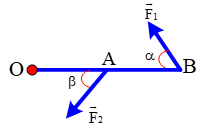
\includegraphics[width=0.25\linewidth]{../figs/VN10-2023-PH-TP0005-8}
	\end{center}
	\begin{mcq}(4)
		\item $\SI{100}{\newton}$.
		\item $\SI{50}{\newton}$.
		\item $\SI{200}{\newton}$.
		\item $\xsi{\dfrac{100}{\sqrt{3}}}{\newton}$.
	\end{mcq}

}
\hideall{
	\textbf{Đáp án B.}\\
Áp dụng quy tắc moment với điểm tựa O:
$$F_1d_1=F_2d_2\Leftrightarrow F_1\cdot OB\sin\SI{30}{\degree}=F_2\cdot OA \Rightarrow F_2=\dfrac{F_1\cdot OB\sin\SI{30}{\degree}}{OA}=\SI{50}{\newton}.$$
}

\item \mkstar{3}\\
Đòn bẩy có cấu tạo như hình \ref{fig:0005-1}. Đầu A của đòn bẩy treo một vật có trọng lượng $\SI{30}{\newton}$. Chiều dài đòn bẩy dài $\SI{50}{\centi\meter}$. Khoảng cách từ đầu A đến trục quay O là $\SI{20}{\centi\meter}$. Cần phải treo một vật khác có trọng lượng bằng bao nhiêu ở đầu B để đòn bẩy cân bằng?
\begin{center}
	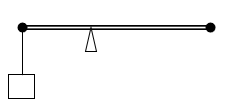
\includegraphics[width=0.35\linewidth]{../figs/VN10-2023-PH-TP0005-1}
	\captionof{figure}{}
	\label{fig:0005-1}
\end{center}
\begin{mcq}(4)
	\item $\SI{15}{\newton}$.
	\item $\SI{20}{\newton}$.
	\item $\SI{25}{\newton}$.
	\item $\SI{30}{\newton}$.
\end{mcq}
\hideall{
	\textbf{Đáp án B.}\\
Áp dụng quy tắc moment với trục quay qua O:
$$P_\text{A}\cdot OA=P_\text{B}\cdot OB\Rightarrow P_\text{B}=\dfrac{P_\text{A}\cdot OA}{OB}=\dfrac{\left(\SI{30}{\newton}\right)\cdot\left(\SI{20}{\centi\meter}\right)}{\SI{30}{\centi\meter}}=\SI{20}{\newton}.$$
}

\item \mkstar{3}\\
Một người dùng búa để nhổ một chiếc đinh. Khi người ấy tác dụng một lực $F=\SI{100}{\newton}$ vào đầu búa thì đinh bắt đầu chuyển động. Lực cản của gỗ tác dụng vào đinh bằng
\begin{center}
	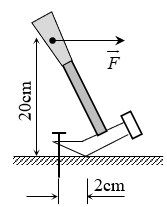
\includegraphics[width=0.15\linewidth]{../figs/VN10-2023-PH-TP0005-2}
\end{center}
\begin{mcq}(4)
	\item $\SI{500}{\newton}$.
	\item $\SI{1000}{\newton}$.	
	\item $\SI{1500}{\newton}$.
	\item $\SI{2000}{\newton}$.
\end{mcq}
\hideall{
\textbf{Đáp án B.}\\
\begin{center}
	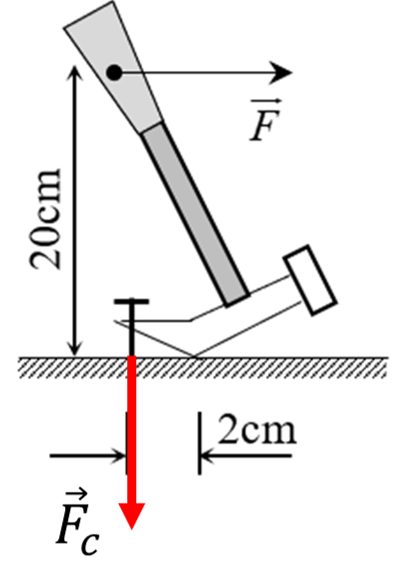
\includegraphics[width=0.15\linewidth]{{../figs/VN10-2023-PH-TP0005-3}}
\end{center}
Áp dụng quy tắc moment với trục quay qua điểm tựa của đầu búa với đất:
$$F\cdot\left(\SI{20}{\centi\meter}\right)=F_c\cdot\left(\SI{2}{\centi\meter}\right)\Rightarrow F_c=10F=\SI{1000}{\newton}.$$
}


\item \mkstar{3}\\
{Một thanh dài $\ell=\SI{1}{\meter}$, khối lượng $m=\SI{1.5}{\kilogram}$. Một đầu thanh được gắn vào trần nhà nhờ một bản lề, đầu kia được giữ bằng một dây treo thẳng đứng. Trọng tâm của thanh cách bản lề một đoạn $d=\SI{0.4}{\meter}$. Lấy $g=\SI{10}{\meter/\second^2}$. Lực căng dây có độ lớn là
	\begin{center}
		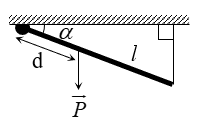
\includegraphics[width=0.25\linewidth]{../figs/VN10-2023-PH-TP0005-4}
	\end{center}
	\begin{mcq}(4)
		\item $\SI{6}{\newton}$.
		\item $\SI{5}{\newton}$.
		\item $\SI{4}{\newton}$.
		\item $\SI{3}{\newton}$.
	\end{mcq}

}
\hideall{
\textbf{Đáp án A.}\\
Áp dụng quy tắc moment cho trục quay qua bản lề:
$$P\cdot d\cdot\cos\alpha=T\cdot\ell\cos\alpha\Rightarrow T=\dfrac{Pd}{\ell}=\SI{6}{\newton}.$$
}

\item \mkstar{3}\\
{Một người nâng một tấm gỗ đồng chất, tiết diện đều, có trọng lượng $P=\SI{200}{\newton}$. Người ấy tác dụng một lực $\vec F$ thẳng đứng lên phía trên vào đầu trên của tấm gỗ để giữ cho nó hợp với mặt đất một góc $\alpha=\SI{30}{\degree}$. Độ lớn lực $F$ bằng 
	\begin{center}
		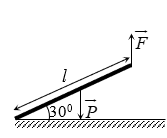
\includegraphics[width=0.25\linewidth]{../figs/VN10-2023-PH-TP0005-5}
	\end{center}
\begin{mcq}(4)
	\item $\SI{100}{\newton}$.
	\item $\SI{86.6}{\newton}$.
	\item $\SI{50}{\newton}$.
	\item $\SI{50.6}{\newton}$.
\end{mcq}
}
\hideall{
\textbf{Đáp án A.}\\
Áp dụng quy tắc moment với điểm tựa là đầu thanh gắn với đất:
$$P\cdot\dfrac{\ell}{2}\cos\SI{30}{\degree}=F\cdot\ell\cos\SI{30}{\degree}\Rightarrow F=\dfrac{P}{2}=\SI{100}{\newton}.$$
}

\item \mkstar{3}\\
{Một người nâng một tấm gỗ đồng chất, tiết diện đều, có trọng lượng $P=\SI{200}{\newton}$. Người ấy tác dụng một lực $F$ vào đầu trên của tấm gỗ (vuông góc với tấm gỗ) để giữ cho nó hợp với mặt đất một góc $\alpha=\SI{30}{\degree}$. Độ lớn lực $F$ bằng 
	\begin{center}
		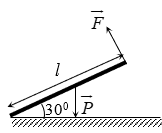
\includegraphics[width=0.25\linewidth]{../figs/VN10-2023-PH-TP0005-6}
	\end{center}
	\begin{mcq}(4)
		\item $\SI{100}{\newton}$.
		\item $\SI{50}{\newton}$.
		\item $\SI{86.6}{\newton}$.
		\item $\SI{50.6}{\newton}$.
	\end{mcq}

}
\hideall{
\textbf{Đáp án C.}\\
Áp dụng quy tắc moment với điểm tựa tại đầu thanh chạm đất:
$$P\cdot\dfrac{\ell}{2}\cos\SI{30}{\degree}=F\cdot\ell\Rightarrow F=\dfrac{P}{2}\cdot\cos\SI{30}{\degree}=\SI{86.6}{\newton}.$$
}

\item \mkstar{4}\\
{Một thanh đồng chất AB, có trọng lượng $P_1=\SI{10}{\newton}$, đầu A được gắn với tường bằng một bản lề, còn đầu B được giữ yên nhờ một sợi dây nằm ngang buộc vào tường tại C. Một vật có trọng lượng $P_2=\SI{15}{\newton}$, được treo vào đầu B của thanh. Cho biết $AC=\SI{1}{\meter}$, $BC=\SI{0.6}{\meter}$. Lực căng dây $T_2$ (dây BC) và $T_1$ (dây treo vật) lần lượt là
	\begin{center}
		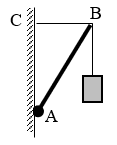
\includegraphics[width=0.15\linewidth]{../figs/VN10-2023-PH-TP0005-7}
	\end{center}
	\begin{mcq}(4)
		\item $\SI{15}{\newton}$; $\SI{15}{\newton}$.
		\item $\SI{15}{\newton}$; $\SI{12}{\newton}$.
		\item $\SI{12}{\newton}$; $\SI{12}{\newton}$.
		\item $\SI{12}{\newton}$; $\SI{15}{\newton}$.
	\end{mcq}

}
\hideall{
\textbf{Đáp án B.}\\
Lực căng dây $T_2$:
$$T_2=P_2=\SI{15}{\newton}$$
Áp dụng quy tắc với điểm tựa A:
$$T_2\cdot BC+P_1\cdot \dfrac{BC}{2}=T_1\cdot CA\Rightarrow T_1=\dfrac{T_2\cdot BC+P_1\cdot \dfrac{BC}{2}}{CA}=\dfrac{\left(\SI{15}{\newton}\right)\cdot\left(\SI{0.6}{\meter}\right)+\left(\SI{10}{\newton}\right)\cdot\left(\SI{0.3}{\meter}\right)}{\SI{1}{\meter}}=\SI{12}{\newton}.$$
}

\item \mkstar{3}\\
{Thanh AB đồng chất có khối lượng $\SI{10}{\kilogram}$. Người ta tác dụng một lực $\vec F$ ở đầu B của thanh như hình vẽ, làm cho thanh bị nâng lên hợp với phương ngang một góc $\SI{30}{\degree}$. Xác định độ lớn của lực $\vec F$, biết $\vec F$ hợp với thanh góc $\SI{60}{\degree}$.
	\begin{center}
		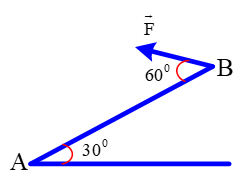
\includegraphics[width=0.25\linewidth]{../figs/VN10-2023-PH-TP0005-9}
	\end{center}
\begin{mcq}(4)
	\item $\SI{100}{\newton}$.
	\item $\SI{50}{\newton}$.
	\item $\SI{200}{\newton}$.
	\item $\SI{150}{\newton}$.
\end{mcq}
}
\hideall{
\textbf{Đáp án B.}\\
Áp dụng quy tắc moment với điểm tựa tại đầu A của thanh:
$$F\cdot d_{\vec F}=P\cdot d_{\vec P}\Leftrightarrow F\cdot AB\sin\SI{60}{\degree}=P\dfrac{AB}{2}\cdot\cos\SI{30}{\degree}\Rightarrow F=\SI{50}{\newton}.$$
}

\item \mkstar{3}\\
{Một vật hình trụ có khối lượng $\SI{10}{\kilogram}$ chịu tác dụng của lực $\vec F$ luôn song song với mặt ngang như hình vẽ. Nếu $h=\dfrac{R}{3}$ thì độ lớn lực $\vec F$ tối thiểu để trụ vượt qua bậc thang là?
	\begin{center}
		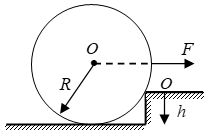
\includegraphics[width=0.25\linewidth]{../figs/VN10-2023-PH-TP0005-13}
	\end{center}
\begin{mcq}(4)
	\item $\xsi{50\sqrt{5}}{\newton}$.
	\item $\xsi{100\sqrt{5}}{\newton}$.
	\item $\xsi{50\sqrt{2}}{\newton}$.
	\item $\xsi{100\sqrt{2}}{\newton}$.
\end{mcq}
}
\hideall{
\textbf{Đáp án A.}\\
\begin{center}
	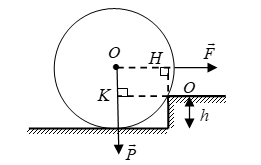
\includegraphics[width=0.3\linewidth]{../figs/VN10-2023-PH-TP0005-14}
\end{center}
Để vật vượt qua bậc thang, ta phải có:
$$M_{F/O_1}\ge M_{P/O_1}$$
$$\Leftrightarrow F\cdot O_1H\ge P\cdot O_1K\Rightarrow F\ge P\cdot\dfrac{O_1K}{O_1H}$$
$$\Rightarrow F\ge P\dfrac{\sqrt{R^2-\dfrac{4}{9}R^2}}{\dfrac{2}{3}R}=\left(\SI{100}{\newton}\right)\cdot\dfrac{\sqrt{5}}{2}=\xsi{50\sqrt{5}}{\newton}.$$
}

\item \mkstar{3}\\
{Một thanh đồng chất khối lượng m có 1 đầu được gắn vào tường bằng bản lề, đầu kia được treo bằng dây nhẹ như hình và thanh cân bằng. Phản lực của bản lề tác dụng vào thanh có phương nào?
\begin{center}
	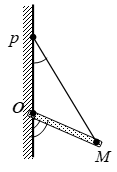
\includegraphics[width=0.15\linewidth]{../figs/VN10-2023-PH-TP0005-11}
\end{center}
\begin{mcq}(2)
	\item Vuông góc với tường.
	\item Phương OM.
	\item Song song với tường.
	\item Có phương hợp với tường một góc nào đó.
\end{mcq}
}
\hideall{
\textbf{Đáp án D.}
}

\item \mkstar{4}\\
{Một ngọn đèn có khối lượng $\SI{2}{\kilogram}$ được treo vào tường bởi sợi dây BC và thanh AB. Thanh AB gắn với tường nhờ vào bản lề A, với AC và BC tạo với nhau một góc $\SI{60}{\degree}$.Tìm lực căng của dây tác dụng lên thanh AB nếu bỏ qua khối lượng thanh. Lấy $g=\SI{10}{\meter/\second^2}$.
\begin{center}
	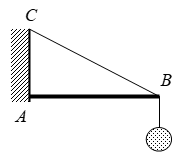
\includegraphics[width=0.25\linewidth]{../figs/VN10-2023-PH-TP0005-12}
\end{center}
\begin{mcq}(4)
	\item $\SI{40}{\newton}$.
	\item $\SI{20}{\newton}$.
	\item $\SI{15}{\newton}$.
	\item $\SI{10}{\newton}$.
\end{mcq}
}
\hideall{
\textbf{Đáp án A.}\\
Áp dụng quy tắc moment với điểm tựa A:
$$P\cdot AB=T\cdot AH=T\cdot AB\sin\SI{30}{\degree}\Rightarrow T=\dfrac{P}{\sin\SI{30}{\degree}}=\SI{40}{\newton}.$$
}

\item \mkstar{4}\\
{Để đẩy một thùng phy nặng có bán kính $R=\SI{3.0}{\centi\meter}$ vượt qua một bậc thềm cao $h<\SI{15}{\centi\meter}$. Người ta phải tác dụng vào thùng một lực $\vec F$ có phương ngang đi qua trục O của thùng và có độ lớn tối thiếu bằng trọng lực $P$ của thùng. Hãy xác định độ cao $h$ của bậc thềm
	\begin{center}
		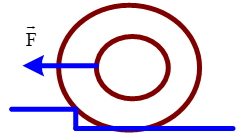
\includegraphics[width=0.25\linewidth]{../figs/VN10-2023-PH-TP0005-10}
	\end{center}
	\begin{mcq}(4)
		\item $\SI{6.3}{\meter}$.
		\item $\SI{8.79}{\meter}$.
		\item $\SI{5.73}{\centi\meter}$.
		\item $\SI{8.25}{\centi\meter}$.
	\end{mcq}

}
\hideall{
\textbf{Đáp án B}\\
Áp dụng quy tắc moment với điểm tựa B:
$$F\cdot d_{\vec F}=P\cdot d_{\vec P}$$
$$\Leftrightarrow F\cdot\left(R-h\right)=P\cdot\sqrt{R^2-\left(R-h\right)^2}$$
Mà $F=P\Rightarrow R-h=\sqrt{R^2-\left(R-h\right)^2}$
$$\Rightarrow h=\SI{8.79}{\centi\meter} \quad \text{hoặc} \quad h=\SI{51.21}{\centi\meter}.$$
Vậy $h=\SI{8.79}{\centi\meter}$ (vì $h<\SI{15}{\centi\meter}$).
}



\end{enumerate}